% NeurIPS 2026 Workshop submission --- "Managing Agents that Manage Agents:
% Responsible Use of Meta-Agents". Non-archival; deadline 2026-08-29 AoE.
%
% STYLE FILE: for the actual submission, download the official
% neurips_2026.sty from the NeurIPS site and drop it beside this file; it is
% then picked up automatically. Until then the fallback below makes the draft
% compile anywhere (Overleaf included) with approximately the right look, so
% the text can be read and edited without waiting on the style file.
% DO NOT SUBMIT the fallback rendering -- the official style controls margins,
% fonts, and the line-numbering/anonymity behaviour reviewers expect.
%
% STATUS MARKERS: \todoresult{} marks a number not yet measured. Every one
% must be resolved or the surrounding claim cut before submission.

\documentclass{article}

\IfFileExists{neurips_2026.sty}{%
  \usepackage[final]{neurips_2026}%
}{%
  % ---- Fallback preamble (official style file absent) -------------------
  \usepackage[margin=1.25in]{geometry}
  \usepackage{natbib}          % neurips_2026.sty normally provides \citep
  \renewcommand{\baselinestretch}{1.02}
  \setlength{\parskip}{2pt}
  \typeout{^^JNOTE: neurips_2026.sty not found -- using draft fallback.^^J}
}

\usepackage[utf8]{inputenc}
\usepackage[T1]{fontenc}
\usepackage{hyperref}
\usepackage{url}
\usepackage{booktabs}
\usepackage{amsfonts}
\usepackage{amsmath}
\usepackage{nicefrac}
\usepackage{microtype}
\usepackage{xcolor}
\usepackage{graphicx}

\newcommand{\todoresult}[1]{\textcolor{red}{[PENDING: #1]}}
\newcommand{\Sz}{\ensuremath{S_0}}
\newcommand{\Sstar}{\ensuremath{S_*}}
\newcommand{\Sevo}{\ensuremath{S_{\mathrm{evo}}}}

\title{Protocol Compliance, Not Capability:\\
What a Self-Improving Coding Agent's Zero Actually Records}

% NOTE: do not begin a line here with a bare "[" directly after "\\" --
% LaTeX parses "\\[...]" as an optional vertical-space argument and fails
% with "Illegal unit of measure". Braces around the placeholders avoid it.
\author{%
  {Author Name} \\
  {Affiliation} \\
  \texttt{author@example.edu}
}

\begin{document}

\maketitle

\begin{abstract}
Self-improving coding agents hold a foundation model frozen and evolve the
scaffold around it, selecting variants by benchmark pass rate. Whether their
reported gains reflect expanded capability or better elicitation remains
unresolved, and any answer presupposes that the selection signal can observe
what the agent does.

We run the unmodified default agent of a published, award-recognised such
system on its own 59-task Polyglot baseline with frozen
\texttt{Qwen2.5-Coder} models. Both 7B and 14B record zero tool calls and
59/59 empty patches, identical in every logged cell. The transcripts
disagree. The 7B model writes prose for a human reader, often in the wrong
language, and closes by explaining how to run it. The 14B model selects the
correct tool and arguments and states its intent to edit the repository, but
emits the call as fenced JSON rather than in the structured field the harness
parses: on 47 of 59 tasks, of which 30 are well-formed enough to dispatch
unchanged. Invalid output formatting is a catalogued tool-use error; its
consequence in this setting is not. Because both failures are recorded as
zero, archive utility is constant and the evolutionary search cannot take its
first step.

Setting \texttt{tool\_choice="required"} restores tool use on 59/59 tasks
($p = 3.4\times10^{-13}$) by constraining decoding to the tool-call grammar,
repairing protocol compliance rather than volition. Pass rate separates none
of this ($2/59$ vs $0/59$, $p = 0.50$) despite a $62\times$ difference in
consumed compute. We report a pre-registered prediction falsified by a
measure we then show was blind to the behaviour it was meant to capture, and
contribute the instrument such attribution requires: matched-compute
elicitation controls, operation tagging by network-layer interception rather
than self-report, causal ablation, and frontier estimation with
non-parametric coverage bounds.
\end{abstract}

\section{Introduction}

A growing line of work treats an agent's \emph{scaffold}---the orchestration
code, prompts, and tool-use policy wrapped around a foundation model---as itself
subject to optimisation. The Darwin--G\"odel Machine
\citep{zhang2025dgm} keeps the foundation model frozen while an outer loop
proposes, evaluates, and archives scaffold variants, each variant's own source
eligible for rewriting by a later generation. Its successors, including the
Huxley--G\"odel Machine \citep{qin2025hgm} and Hyperagents
\citep{zhang2026hyperagents}, refine the search and report substantial gains:
DGM improves SWE-bench performance from 20.0\% to 50.0\% and Polyglot from
14.2\% to 30.7\%.

These deltas are ambiguous in a specific, consequential way. A scaffold can
raise measured pass rate through at least three routes that involve the frozen
model doing nothing it could not already do:

\begin{enumerate}
\item \textbf{Elicitation.} Better prompting, retries, or sampling surface an
  answer the model could always produce but rarely samples.
\item \textbf{Benchmark overfitting.} The scaffold specialises to the specific
  verifier used for selection rather than the underlying task.
\item \textbf{Search.} Best-of-$N$ selection and execution feedback do real work
  that is a property of the \emph{search procedure}, not of the model's
  capability boundary.
\end{enumerate}

None of these is self-improvement in the sense the framing implies, and
aggregate pass-rate comparison (current practice) cannot distinguish them from
genuine capability expansion.

Our central empirical claim (Section~\ref{sec:results}) is not that a
tool-policy flag changes tool use, which is definitional, but three
things that are not:

\begin{enumerate}
\item A \emph{published, award-recognised} system's own default agent records
  \textbf{zero tool calls} on \emph{its own} benchmark at both 7B and 14B
  scale: 59/59 empty patches, six languages, no exception. Every quantity
  the system logs is identical across the two scales.
\item \textbf{That zero conceals two unrelated failures.} The transcripts
  show the 7B model writing prose for a human reader, and the 14B model
  selecting the correct tool and arguments but emitting the call in the
  wrong channel---fenced JSON rather than the structured field the harness
  parses. On 30/59 tasks the 14B call is well-formed enough to have been
  dispatched by a lenient parser. We had registered the prediction that 14B
  would show non-zero tool use and scored it falsified; we report that the
  falsification was an artifact of measuring structured
  \texttt{tool\_calls} alone.
\item \textbf{No selection signal in use can separate these cases.} Two
  configurations differing totally in behaviour and $62\times$ in compute
  are statistically indistinguishable in pass rate, so a search optimising
  it cannot distinguish an agent that never tries from one that is a
  serialisation format away from acting.
\end{enumerate}

\paragraph{Two contributions, and their present status.}
This paper contributes an \emph{instrument} and a \emph{result obtained
while validating it}, and we state the relationship between them plainly
because it determines what may be concluded from either.

The instrument (\S\ref{sec:instrument}) is a measurement layer for
attributing a self-improving system's gains between elicitation and
capability expansion. It comprises a scaffold ladder with a matched-compute
elicitation control, operation tagging enforced by network-layer
interception rather than agent self-report, causal ablation that withholds
an information channel rather than requesting its disuse, and frontier
estimation with non-parametric coverage bounds. It is designed to attach to
an existing, independently-implemented loop rather than to a system
co-designed with its own evaluation.

\textbf{It is not yet fully validated, and we do not claim it is.} The
interception layer is exercised here at scale ($1.28\times10^4$ intercepted
calls) and is what produced the result below. The elicitation control is
implemented and partially run; causal ablation and frontier estimation are
implemented and unit-tested but have not been run against a real evolved
scaffold, because---as \S\ref{sec:results} shows---no evolved scaffold could
be produced in this configuration. A component that has not met real data is
reported as such throughout.

The result (\S\ref{sec:results}) is what the interception layer found when
pointed at the baseline: a recorded zero that conceals two unrelated
failures, one of them a serialisation error that halts the search
mechanically. We regard the result as the more secure of the two
contributions, since it rests on measurements rather than on a design.
\S\ref{sec:repro} reports separately on executing the \emph{proposal} half
of the same system, where six defects had to be repaired before a scaffold
variant could be generated at all, and four of the six were reported through
the same channel as ordinary model failure.

\section{Related work}

\paragraph{Self-improving coding agents.}
DGM \citep{zhang2025dgm}, HGM \citep{qin2025hgm}, Hyperagents
\citep{zhang2026hyperagents}, and SICA \citep{robeyns2025sica} all report
frozen-model scaffold evolution with substantial benchmark gains. None
independently estimates the frozen model's own ceiling under repeated sampling,
and none tests an elicitation alternative at matched compute. Hyperagents
explicitly lists fixed evaluation protocols as a limitation.

The comparison structure is worth stating precisely, since HGM is both the
strongest result in this family and the system we fork. Its evaluation compares
three \emph{evolutionary} methods (SICA, DGM, and HGM) from an identical
initial agent. The sole human-engineered reference point is a leaderboard
comparison against SWE-agent \citep{yang2024sweagent}, which uses a different
backbone at an unmatched compute budget. There is therefore no condition in
which the frozen backbone is measured without an evolving scaffold, and no
fixed-scaffold control at matched compute. The reported gain is real; what it
is a gain \emph{over} is a moving scaffold, not a characterised model ceiling.

\paragraph{Evaluation of self-evolving agents.}
Recent benchmarks target adjacent axes: EvoAgentBench
\citep{gao2026evoagentbench} measures transfer of extracted ``abilities''
across model families; SEA-Eval \citep{seaeval2026} measures success rate
against token cost over sequential task streams. On the basis of their
abstracts and summaries (we have not yet read either in full), neither
appears to estimate a frozen-model frontier or to attribute gains between
elicitation and expansion.

\paragraph{Tool-use error taxonomies.}
The failure we characterise in Section~\ref{sec:results} is a known one.
\citet{kokane2024toolscan} catalogue seven recurring tool-use error patterns
in LLMs, among them \emph{invalid output formatting}, which covers models
that emit a call as markdown or unstructured JSON rather than in the
structured field a harness parses. \textbf{We claim no novelty for the
phenomenon.} What is new here is its consequence in a setting that taxonomy
does not consider: inside a self-improving system, a formatting failure does
not merely lower a score, it drives the selection signal to a constant and
halts the search that consumes it. \citet{kokane2024toolscan} evaluate
tool-use accuracy directly and do not connect these errors to benchmark
selection signals or to evolutionary agent systems; that connection, and its
consequences for attribution, is our contribution.

\paragraph{Elicitation gaps.}
Work on scaffold-induced performance variation \citep{starace2026scaffold}
and on capability elicitation as a lower bound \citep{metr2025horizon} supplies
the framing and statistical machinery we extend, but studies \emph{static}
scaffolds. Closest to our attribution question, \citet{iscan2026placebo}
run placebo-controlled decompositions of execution-feedback self-repair in
frozen small code models, finding feedback's advantage over a content-free
placebo statistically indistinguishable from zero---but for a fixed retry loop,
with no frontier-crossing concept.

Table~\ref{tab:gap} summarises the gap.

\begin{table}[t]
\caption{Methodological coverage in closely related work. Entries record
whether each paper's \emph{own reported evaluation} includes the control,
not whether its authors would consider it necessary. Verification basis is
stated explicitly because these are claims about absence: HGM, SICA,
Hyperagents and \citet{iscan2026placebo} were checked against full text;
$\dagger$ marks papers assessed from abstract and summary only at time of
writing, where absence should be read as ``not found'' rather than
``confirmed absent''.}
\label{tab:gap}
\centering
\small
\begin{tabular}{lccccc}
\toprule
& Frozen-model & Matched-compute & Intercepted & Causal & Pre- \\
& ceiling & elicitation ctrl. & attribution & ablation & registered \\
\midrule
DGM              & --- & --- & --- & --- & --- \\
HGM              & --- & --- & --- & --- & --- \\
Hyperagents      & --- & --- & --- & --- & --- \\
SICA             & --- & --- & --- & --- & --- \\
EvoAgentBench$\dagger$ & --- & --- & --- & --- & --- \\
SEA-Eval$\dagger$      & --- & --- & --- & --- & --- \\
\citet{iscan2026placebo} & \checkmark & \checkmark\,(static) & --- & --- & \checkmark \\
\midrule
\textbf{This work} & \checkmark & \checkmark & \checkmark & \checkmark & \checkmark \\
\bottomrule
\end{tabular}
\end{table}

\section{Instrument}
\label{sec:instrument}

\paragraph{Scaffold ladder.}
\Sz{} is the minimal scaffold (one trajectory, no retries, no selection), and
by construction \emph{defines} the frontier against which everything else is
measured. \Sstar{} is a strong, fixed, hand-authored baseline (best-of-$N$,
execution feedback against public tests only, tool use, self-consistency). Its
role is to answer the elicitation question directly: how much of any observed
gain is reachable \emph{without evolution at all}, at matched compute. \Sevo{}
is a forked, independently-implemented evolving scaffold.

The ladder is deliberately ordered by what each rung licenses. A gain over
\Sz{} shows only that the scaffold does something; a gain over \Sstar{} at
matched compute is the first result that cannot be explained by sampling the
same frozen model harder. We treat the second comparison, not the first, as
the meaningful one, and report both.

\paragraph{Attribution by interception, not self-report.}
An evolved scaffold's code is produced by a process optimising ``solve more
tasks,'' not ``report your own operations honestly''; a variant that omitted
tagging an expanding operation would face no pressure against doing so. We
therefore never rely on instrumentation \emph{inside} the agent. Because
forked agents run as separate OS processes inside Docker, we intercept at the
only remaining boundary, the network, using a transparent reverse proxy
between container and model server that records every request/response pair.
Operations are then classified post hoc from what was observed.

Two properties of this design matter for what the paper can claim. First, the
proxy observes the wire, so it sees exactly what the harness sees and nothing
more: this is what let us establish that the \texttt{auto} arms issue one
generation per task, and equally what prevented us from noticing, until we
read trajectories, that a majority of those generations \emph{contained} a
tool call. An interception layer is an honest witness to the protocol, not to
intent, and \S\ref{sec:results} is in part a report of that distinction
mattering. Second, non-200 responses are recorded but excluded from
generation counts, so a backend error cannot inflate a scaffold's apparent
work; we found this necessary after an early version counted failed calls as
legitimate generations.

Each intercepted operation is labelled \emph{support-preserving} (selection,
retries, self-consistency: replicable by sampling the frozen model harder) or
\emph{support-expanding} (tool output conditioning later generations,
execution feedback reshaping a prompt). The partition is the load-bearing
abstraction of the instrument: support-preserving operations cannot move the
frozen model's reachable set by construction, so a gain attributable
entirely to them is elicitation regardless of how large it is. Classification
is behavioural---whether a later request contains a substantial fragment of
an earlier response or of execution output---and we treat it as evidence
rather than proof (\S\ref{sec:limitations}).

\paragraph{Compute accounting.}
Every model call is charged to a budget accountant that records prompt and
completion tokens, so ``matched compute'' is a measured quantity rather than
a nominal setting. This is what makes the elicitation control meaningful: a
scaffold that wins by issuing sixty times more generations has not
demonstrated anything about the model. For containerised trajectories the
charge is necessarily post hoc, since a trajectory's cost is not known until
it has run, so the accountant surfaces overruns rather than preventing them.

\paragraph{Causal ablation.}
To test whether a support-expanding operation is \emph{necessary} for a solve,
we withhold the information channel itself rather than instructing the agent
not to use it---an ablated agent is denied the capability regardless of what
its own code attempts.

\paragraph{Frontier estimation.}
Per-task success rates use Clopper--Pearson exact intervals; coverage of the
unseen difficulty distribution uses Good--Turing and Chao1. A central
discipline: the estimator cannot express $p = 0$. Every ``beyond frontier''
record carries an explicit budget-relative qualifier.

\paragraph{Pre-registration.}
Thresholds, the bootstrap procedure, multiple-comparison correction, and the
interpretation matrix were fixed before any evolutionary result existed. The
sub-study reported below was likewise declared---including its predictions and
the manipulation---before its runs executed.

\section{Scaffold sensitivity: a cautionary result}
\label{sec:results}

\subsection{Setup}

\paragraph{Tasks and grading.}
We run \Sz{} on the 59-task Polyglot subset that HGM itself uses as its
baseline evaluation set,\footnote{HGM's own subset definition lists 60 entries,
of which 59 are unique; one instance identifier appears in both of its
constituent files.} spanning six languages (C++, Go, Java, JavaScript, Python,
Rust); the full list is given in Appendix~\ref{app:tasks}. Choosing the
system's own subset is deliberate: a null result on a set we selected would
invite the objection that we chose unfavourable tasks.
Grading uses HGM's real harness rather than a reimplementation: a per-task
Docker container in which the hidden tests are revealed, by resetting to a
test commit, only after the agent has stopped. The agent therefore never sees
the tests it is graded on, and we inherit the harness's own definitions of
\texttt{resolved}, \texttt{unresolved}, and \texttt{empty\_patch}.

\paragraph{Model and serving.}
The frozen models are \texttt{Qwen2.5-Coder-7B-Instruct} and
\texttt{Qwen2.5-Coder-14B-Instruct-AWQ} (4-bit weight quantisation, used so
the larger model fits the same single 24\,GB accelerator and the scale
comparison costs no additional hardware). Both are self-hosted under vLLM
0.26 with a 16{,}384-token context, automatic tool-choice parsing enabled and
the model family's own tool-call parser selected. Self-hosting is
load-bearing: it makes frozen-ness verifiable rather than promised, keeps
contamination questions inspectable, and matters because frontier estimation
is sample-hungry. It is also what surfaces the result in
\S\ref{sec:results}---a hosted endpoint that silently repaired malformed tool
calls would have hidden the failure entirely.

The \texttt{required} arms differ from the \texttt{auto} arms in exactly two
source lines, both in the agent's own model-call wrapper, applied to an
isolated copy so the measured default agent is never mutated. All other
configuration is byte-identical, including sampling parameters, and each
result record carries the model identifier and agent-variant name so that no
two arms can be merged by accident.

\paragraph{Deviation for the self-improvement runs.}
The runs in \S\ref{sec:repro} required a 32{,}768-token context, because
HGM's diagnosis prompt does not fit a 16k window. Those runs therefore do
\emph{not} share a serving configuration with the four arms reported in
Table~\ref{tab:main}, and we do not compare their numbers directly; each
re-evaluates its own seed. We state this rather than quietly pool the two.

We manipulate one variable: the agent's \emph{tool policy}, set by the
\texttt{tool\_choice} parameter of the OpenAI-compatible chat API. The
parameter takes three named values: \texttt{"none"}, under which the model
may not call a tool; \texttt{"auto"}, under which the model decides for
itself whether to call one; and \texttt{"required"}, under which it must
emit at least one call, enforced by constraining decoding to the tool-call
grammar. HGM's released agent uses \texttt{"auto"}. We write these values
literally rather than paraphrasing them, because the distinction between
``the model chose not to call a tool'' and ``the model could not emit a
call in the required form'' is what Section~\ref{sec:results} turns on, and
a gloss such as \emph{optional} would blur it.

Throughout, we label the two conditions the \textbf{\texttt{auto} arm} and
the \textbf{\texttt{required} arm}. The \texttt{required} variant differs
from HGM's unmodified default agent in \textbf{exactly two lines}, both the
\texttt{tool\_choice} flag; we verify this by direct diff rather than
assertion. All other scaffold code, the model, the task set, and the grading
harness are identical.

\subsection{Results}

\IfFileExists{fig1_asymmetry.pdf}{%
\begin{figure}[t]
\centering
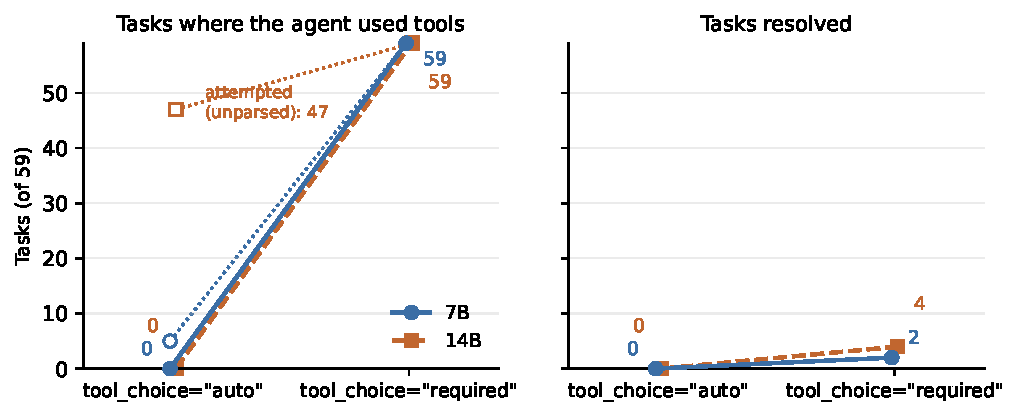
\includegraphics[width=\linewidth]{fig1_asymmetry.pdf}
\caption{The same two-line scaffold change, measured three ways, on a shared
$0$--$59$ axis. Left, filled markers: tasks with a \emph{structured} tool
call, the quantity the harness acts on. Left, hollow markers: tasks where a
tool call was \emph{attempted}, counted from the transcripts. Right: tasks
resolved. The gap between hollow and filled at
\texttt{tool\_choice="auto"}---47 versus 0 for the 14B model---is the
measurement artifact this paper reports: the two scales are identical in
every recorded cell while differing almost tenfold in attempted actions.
Plotting all panels on one scale is deliberate; on its own axis the
resolve-rate panel would suggest a large effect, which is the misreading we
argue against.}
\label{fig:asymmetry}
\end{figure}}{}

\begin{table}[t]
\caption{\Sz{} on the 59-task Polyglot baseline. ``Used tools'' counts tasks
with at least one intercepted tool call. Intervals are Clopper--Pearson 95\%.}
\label{tab:main}
\centering
\small
\begin{tabular}{lrrrrr}
\toprule
Arm & $n$ & Resolved & Used tools & Tool calls & Generations \\
\midrule
7B $\times$ \texttt{auto}      & 59 & 0 \,[0.000, 0.061] & 0 \,[0.000, 0.061] & 0 & 59 \\
7B $\times$ \texttt{required}  & 59 & 2 \,[0.004, 0.117] & \textbf{59} \,[0.939, 1.000] & 3663 & 3687 \\
14B $\times$ \texttt{auto}     & 59 & 0 \,[0.000, 0.061] & 0 \,[0.000, 0.061] & 0 & 59 \\
14B $\times$ \texttt{required} & 59 & 4 \,[0.019, 0.165] & \textbf{59} \,[0.939, 1.000] & 5592 & 5617 \\
\bottomrule
\end{tabular}
\end{table}

\paragraph{Behaviour under the default policy.}
Under HGM's unmodified \texttt{tool\_choice="auto"} default, both frozen models
resolved \textbf{0 of 59} tasks and made \textbf{0 tool calls}, uniformly across
all six languages. The uniformity is total: at both scales the distribution of
per-task model calls is $\{1\}$, of tool calls $\{0\}$, and of produced patch
lengths $\{0\}$. Not one task deviated. Neither model is failing at code; each
emits several hundred tokens of coherent analysis (7B mean 902, 14B mean 976)
before terminating with \texttt{finish\_reason="stop"} and
\texttt{tool\_calls=None}. Since no file is modified, the diff is empty and the
task fails before any test executes.

\paragraph{The zero conceals two unrelated failures.}
Read only through the API, the two scales are indistinguishable. Read through
the transcripts, they are doing different things, and only one of them
resembles the natural reading of a zero.

The 7B model does not appear to model itself as the actor. It writes a
solution for a human reader and closes by explaining how that reader might
install it (Figure~\ref{fig:transcripts}, top). It holds an edit tool
throughout and has been told it is operating on a repository.

The 14B model does the opposite. It behaves as an agent, names the tool it
intends to use, selects arguments correctly, and then emits the call as fenced
JSON in the assistant message rather than in the structured field the harness
parses (Figure~\ref{fig:transcripts}, bottom). We verified that this is not a
deployment fault: the chat template renders the full tool schemas inside
\texttt{<tools>} tags and states the required
\texttt{<tool\_call>}\ldots\texttt{</tool\_call>} convention with a worked
example, and an identical request differing only in
\texttt{tool\_choice="required"} returns the same intent as a structured call.
The model is told the protocol and does not follow it. Appendix
\ref{app:protocol} records these checks in full, since the alternative
explanation---that our deployment failed to advertise the tools---would
invalidate the result entirely.

Table~\ref{tab:prose} quantifies this over all 118 transcripts. We grade
each at three strictnesses, since they license different claims: whether a
call was \emph{emitted} at all, whether it \emph{parses} as JSON, and whether
it is \emph{runnable}, meaning it names a real tool and supplies every
required argument, so a lenient parser could have dispatched it unchanged.

\begin{figure}[t]
\centering
\small
\begin{minipage}{0.95\linewidth}
\textbf{(a) 7B, \texttt{python\_\_dominoes}} --- the model addresses a human
reader.
\begin{quote}\itshape\footnotesize
``To integrate this into your project, you can create a new Python file in the
\texttt{/testbed/} directory, say \texttt{domino\_solver.py}, and add the above
code to it. Then, you can call this function from your main
program\ldots{} If you need further assistance or have additional
requirements, feel free to let me know!''
\end{quote}
\rule{\linewidth}{0.4pt}
\textbf{(b) 14B, \texttt{cpp\_\_all-your-base}} --- the model acts, in the
wrong channel.
\begin{quote}\itshape\footnotesize
``Now, let's apply these changes to the code files in the \texttt{/testbed/}
directory. We'll use the \texttt{editor} tool to edit the
\texttt{base\_converter.py} file.''
\end{quote}
\begin{quote}\ttfamily\footnotesize
\{"name": "editor", "arguments": \{"command": "edit",\\
"path": "/testbed/base\_converter.py", "file\_text": "\ldots"\}\}
\end{quote}
\end{minipage}
\caption{Assistant output from the two \texttt{auto} arms; both responses
carry \texttt{tool\_calls=None} and are scored identically as
\texttt{empty\_patch}. In (b) the call names a real tool with valid
arguments and is emitted as fenced JSON rather than inside
\texttt{<tool\_call>} tags. Note also that (b) targets a Python file for a
C++ task, the wrong-artifact mode of \S\ref{sec:results}.}
\label{fig:transcripts}
\end{figure}

\begin{table}[t]
\caption{Tool calls in the \texttt{auto} arms, graded by strictness.
``Structured'' is what the harness reads and what Table~\ref{tab:main}
reports. ``Runnable'' calls are dispatchable as-is; this is not a claim that
the task would then have been solved.}
\label{tab:prose}
\centering
\small
\begin{tabular}{lrrrr}
\toprule
Arm & Structured & Emitted & Parses & Runnable \\
\midrule
7B $\times$ \texttt{auto}  & 0/59 & 5/59  & 2/59  & 1/59 \\
14B $\times$ \texttt{auto} & 0/59 & \textbf{47/59} & 38/59 & \textbf{30/59} \\
\bottomrule
\end{tabular}
\end{table}

On \textbf{30 of 59} tasks the 14B agent is a serialisation format away from
proceeding, and the harness records that outcome as identical to the 7B
agent's conversational misunderstanding. The attrition between columns is
itself informative: nine emitted calls are malformed JSON and a further eight
parse but omit a required argument, so the model's protocol failure is
graded rather than absolute.

The effect is not an artifact of one language's task phrasing. Table
\ref{tab:bylang} breaks the same measurement down by language: the 14B model
attempts a call in every one of the six, at rates between $6/10$ and $10/10$,
while the 7B model attempts almost none anywhere. The two models differ
consistently, and neither differs much across languages.

\begin{table}[t]
\caption{Attempted (emitted) and dispatchable (runnable) tool calls per
language in the \texttt{auto} arms. Structured tool calls are $0$ in every
cell of this table, for both models and all six languages.}
\label{tab:bylang}
\centering
\small
\begin{tabular}{lrrrrr}
\toprule
& & \multicolumn{2}{c}{14B $\times$ \texttt{auto}} & \multicolumn{2}{c}{7B $\times$ \texttt{auto}} \\
\cmidrule(lr){3-4}\cmidrule(lr){5-6}
Language & $n$ & Emitted & Runnable & Emitted & Runnable \\
\midrule
C++        & 5  & 5  & 2 & 0 & 0 \\
Go         & 10 & 10 & 7 & 0 & 0 \\
Java       & 12 & 8  & 4 & 1 & 0 \\
JavaScript & 10 & 6  & 5 & 1 & 1 \\
Python     & 11 & 8  & 4 & 3 & 0 \\
Rust       & 11 & 10 & 8 & 0 & 0 \\
\midrule
Total      & 59 & \textbf{47} & \textbf{30} & 5 & 1 \\
\bottomrule
\end{tabular}
\end{table}

\paragraph{Effect of the tool-policy flag.}
That setting \texttt{tool\_choice="required"} increases tool calls is
definitional, and the mechanism matters for how the result may be read. Under
this setting the serving stack constrains decoding to the tool-call grammar,
so a structured call is emitted whether or not the model would have produced
one unprompted. Given Table~\ref{tab:prose}, the honest description is that
the flag \textbf{repairs protocol compliance}, not that it induces volition:
for the 14B model, intent was already present in a majority of transcripts
and only the serialisation was wrong. \emph{We therefore do not claim that
the tool policy determines whether the agent tries to act.} What we claim is
narrower and sufficient: the flag determines whether the harness can
\emph{observe} an attempt, and every selection signal in use depends on that
observation.

Three consequences are not definitional, and are what we report: the measured
baseline is exactly zero rather than merely low; the same flag separates
``this system does nothing'' from ``this system solves tasks'' on a benchmark
the system's authors chose; and the change is invisible to pass rate. A flag
whose behavioural effect is definitional can still be undetectable at the
level a search actually optimises, and that gap is the finding.

Switching \texttt{tool\_choice} from \texttt{"auto"} to \texttt{"required"},
with everything else byte-identical, moves the 7B agent from 0 tool calls to
3663 across the same 59 tasks---every single task using tools, in every
language ($59/59$, Fisher exact $p = 3.4\times10^{-13}$). Model calls rise
from 59 to 3687, and the agent now produces real patches that receive real
test verdicts: 53 of 59 tasks yield a non-empty diff, and the modal outcome
changes from \texttt{empty\_patch} (59/59) to \texttt{unresolved} (51/59).
Two tasks are solved outright. The 14B model behaves the same way under the
same flag (5592 tool calls, 4 solved), so the effect is a property of the
policy, not of a particular model. Figure~\ref{fig:asymmetry} plots both
measurements on a common axis: the same intervention that saturates the
behavioural panel barely lifts the resolve-rate panel off zero.

\paragraph{A pre-registered prediction, its falsification, and a defective
measure.}
Before running the larger-model arms we registered the prediction that
\texttt{14B}~$\times$~\texttt{auto} would show non-zero tool use---i.e.\ that
the floor reflected a capability threshold the 7B model sat below. We
operationalised ``tool use'' as structured \texttt{tool\_calls}, the quantity
the harness itself acts on. Against that measure the prediction was falsified
outright: \texttt{14B}~$\times$~\texttt{auto} produced \textbf{0/59 resolved,
0/59 tasks with any tool call, and 59/59 empty patches}, identical to the 7B
arm in every cell, including the distributions of per-task generations
($\{1\}$) and patch lengths ($\{0\}$), with mean completion tokens rising
only from 902 to 976.

\textbf{We report the falsification as it was scored, and we also report that
the measure was inadequate.} Table~\ref{tab:prose} shows the prediction's
substance---that the larger model would attempt to use tools---was in fact
correct, and by a wide margin (47/59 versus 5/59 attempted calls); it was the
operationalisation that could not see it. Both facts belong in the record.
Registering the prediction is what forced the transcripts open: had we not
written it down, the post-hoc framing ``a 7B model is too weak to be an
agent'' would have been available, comfortable, and wrong, and the
identical-in-every-cell result would have looked like confirmation of it.

We draw the methodological point rather than soften it. A pre-registered
measure can be wrong in the same way a scaffold's selection signal can be
wrong, and for the same reason: both were defined over what the system
records rather than what the agent does.

\paragraph{A third failure mode: acting on the wrong artifact.}
Forcing tool use does not make the agent competent at the task
\emph{interface}. In 9 of 59 cases in the 14B \texttt{required} arm, the agent
worked productively (tens to hundreds of tool calls) but created a
\emph{new file of its own naming} rather than editing the exercise's declared
solution files. Frequently the new file was in the wrong language entirely:
\texttt{diamond\_kata.py} for the C++ task \texttt{cpp\_\_diamond},
\texttt{robot.py} and \texttt{spell\_number.py} for JavaScript tasks. The
harness stashes only the declared solution paths before revealing the hidden
tests, so these attempts leave nothing gradeable behind:

\begin{quote}\small\ttfamily
No local changes to save\\
HEAD is now at 632858f\\
Removing diamond\_kata.py\\
No stash entries found.
\end{quote}

We count these as unresolved rather than excluding them, since the task was
certainly not solved; excluding them would inflate the resolve rate by
shrinking the denominator over exactly the attempts that failed. The mode is
worth naming because it is a third way the scaffold--model interface, not the
model's coding ability, determines the measured outcome---and because it too
is invisible in a pass-rate column, where it is indistinguishable from having
tried and been wrong.

\subsection{Implications}

\paragraph{The recorded quantity is not the phenomenon.}
The central consequence is not that a flag changes behaviour---that is
definitional---but that a single recorded value, $0$ tool calls, covers two
unrelated states of the system. In one, the model does not act. In the other
it selects the correct tool and arguments and fails to serialise them. Every
quantity HGM logs is identical across the two: resolve count, tool-call
count, patch length, and the per-task distributions of each. The distinction
is recoverable only from trajectories, which no selection procedure in this
family reads.

This is what the tool-policy manipulation is for, and it is worth being
precise about its role. It is not the finding; it is the control that
establishes the finding's direction. Because constraining decoding to the
tool-call grammar converts the same model, on the same tasks, from $0$ to
$59/59$ tasks using tools, the deficit under the default policy cannot be
attributed to an inability to determine \emph{what} to do. The 14B
transcripts show the intended call already formed
(Table~\ref{tab:prose}); the constrained-decoding arm shows the same intent
surviving into the structured field. What separates them is a wire format.

\paragraph{Why this is not merely a scoring inaccuracy.}
An evaluation error that lowered all scores uniformly would be a nuisance.
This one is structural, because self-improving systems consume their own
scores. HGM samples archive nodes of \emph{strictly positive} utility before
expanding one. A protocol failure sends every node to zero, the candidate
set is empty for every node, and the search cannot take its first step---the
implementation raises \texttt{ValueError: attempt to get argmax of an empty
sequence}. The formatting failure does not degrade the search; it prevents
it from starting. We observed exactly this, and it is why the evolutionary
run reported in \S\ref{sec:repro} required a seed configuration that scores
above zero at all.

\paragraph{Scaffold policy versus model scale.}
The claim here is regime-relative: what follows holds for the
two model scales, one task family, and one forked system tested here, and we
do not claim scaffold dominates model capability in general. Within that
scope, model scale predicts recorded agentic behaviour not at all under the
default policy ($0/59$ vs $0/59$, $p = 1.0$), while predicting
\emph{attempted} behaviour strongly ($47/59$ vs $5/59$). Resolve rate never
reaches significance in any comparison ($0$, $2$, $0$, $4$ of 59; smallest
$p = 0.12$). For meta-agent evaluation this reverses the usual attribution:
a harness search that stumbles onto a tool-policy change is not discovering
a better agent, it is discovering the switch that makes the agent's actions
legible---and it will be credited with a capability gain either way.

\paragraph{Frontier degeneracy.}
\Sz{} is what defines the measurable frontier. When $\Sz{} = 0$, every condition
of a frontier-crossing test becomes vacuous: there is no task \Sz{} plausibly
fails-but-could-solve, the estimator has nothing to estimate, and \emph{any}
nonzero evolved-scaffold result crosses trivially. This is an
\emph{uninformative} null: the instrument could not have detected an
effect, which is categorically weaker than a well-powered null. We flag this
because a study that reported ``the evolved scaffold beat the baseline'' from
exactly this configuration would be reporting an artifact.

\paragraph{What a scaffold search would be rewarded for.}
The interventions that move this system's measured score are not ones that
change what the frozen model can do. Repairing serialisation moves it from
$0/59$ to $4/59$ with the weights untouched by construction; so, plausibly,
would a prompt line specifying which file to edit, given that 9/59 of the
tool-using runs failed by writing an undeclared file
(\S\ref{sec:results}). Both are interface repairs. Both would be credited as
capability gains under current evaluation practice, because pass rate is
the only thing being read. The concern is not that a search might find such
a change---finding it is useful---but that nothing in the reported
methodology distinguishes having found it from having improved the agent.

\paragraph{Compute is reported, not matched.}
We report compute rather than equalising it, because equalising is not
meaningful here: an agent that never acts cannot spend a comparable budget.
The \texttt{auto} arms issue exactly one generation per task (59 total); the
7B \texttt{required} arm issues 3687, a $62\times$ increase, with mean
completion tokens per task rising from 902 to 6637. So the arms differ not
only in behaviour but in consumed compute by nearly two orders of
magnitude---and are still statistically indistinguishable in the utility a
pass-rate objective assigns them ($p = 0.50$). A selection procedure that
cannot separate scaffolds differing by $62\times$ in compute and totally in
behaviour is not measuring what its users believe it measures.

\paragraph{Behavioural effect versus pass-rate effect.}
The difference in
whether the agent \emph{acts at all} is about as decisive as a $2\times2$ table
can be: \textbf{59/59 versus 0/59} tasks with at least one tool call, Fisher
exact $p = 3.4\times10^{-13}$, with non-overlapping Clopper--Pearson intervals
($[0.939, 1.000]$ vs $[0.000, 0.061]$) and no exceptions in any of the six
languages. The difference in tasks \emph{resolved} is not: 2/59 versus 0/59
yields $p = 0.50$, and at $n = 59$ per arm this design cannot detect a
resolve-rate shift smaller than roughly $6/59$ at $\alpha = 0.05$. We therefore
do \textbf{not} claim that changing the tool policy improves pass rate. It
changes behaviour categorically and moves resolve rate off the floor by a
margin this experiment is underpowered to certify.

\paragraph{A blind spot in pass-rate selection.}
Combining the behavioural and pass-rate findings: the arms differ by
$p\approx10^{-13}$ in whether the agent acts, and are indistinguishable in the
signal used to select between them. A search procedure optimising pass
rate, as DGM, HGM, and SICA all do, receives almost no gradient from the
single change that determines whether its agent is an agent. The scaffold
change that would break the deadlock is precisely the one its objective cannot
see.

\paragraph{An interpretability band.}
The base model must be strong enough that the selection signal is
non-degenerate, but the scaffold must already be functional enough that the
search is not merely rediscovering its own switches. Neither boundary is
currently reported by any system we reviewed.

\paragraph{A concrete consequence for meta-agent evaluation.}
Reported gains for self-improving agents should be accompanied by (i) an
independent estimate of the frozen model's own ceiling under repeated sampling,
and (ii) a fixed-scaffold elicitation control at matched compute. Without both,
a pass-rate delta is consistent with the model's capability boundary not having
moved at all.

\section{Executing the self-improvement path}
\label{sec:repro}

The results above concern the \emph{evaluation} half of a self-improving
system. We also attempted its \emph{proposal} half, forking HGM and running
\texttt{sample\_child}---the routine that generates a scaffold variant---against
our self-hosted deployment. To our knowledge this path had not previously been
exercised outside its authors' own hosted configuration, and six defects had to
be repaired before a single child could be proposed. We report them because the
distribution of \emph{how they surface} is itself a finding, not because any
individual defect is interesting.

\textbf{We report no evolutionary result, and state the scope precisely so
that none is inferred.} After the repairs below, a two-task configuration
ran the loop end to end: two children were proposed, archived, and
evaluated, which establishes that the path executes. A full 59-task run then
completed its seed evaluation---the seed scores $4/59$, matching the
\texttt{14B} $\times$ \texttt{required} arm's rate on three of the same four
tasks---but was halted during its first \texttt{sample\_child} call before
any child was archived. What follows is therefore an account of making the
proposal half runnable, not a measurement of what it proposes. The
attribution study the instrument was built for remains unrun.

\begin{table}[t]
\caption{Defects encountered before the self-improvement path would execute.
The final column is the point: only two announce themselves. The remainder
are reported through the same channel as ordinary model failure, so a study
that read summary statistics rather than container logs would have recorded
them as the agent performing badly.}
\label{tab:repro}
\centering
\small
\begin{tabular}{p{0.46\linewidth}p{0.20\linewidth}p{0.26\linewidth}}
\toprule
Defect & Location & How it surfaces \\
\midrule
Self-improvement container created without host networking, so the agent
cannot reach the model server &
container setup &
Crash (loud) \\
\addlinespace
Build staging reused across runs; \texttt{copytree} cannot overwrite git's
read-only objects &
image build &
Task marked failed \\
\addlinespace
Exception handler references an unassigned variable, raising a second error
that replaces the first &
child sampling &
Wrong cause reported \\
\addlinespace
Seed directory copied \emph{into} an existing output directory rather than
replacing it, so a rerun reads its predecessor's metadata &
run initialisation &
Silently wrong numbers \\
\addlinespace
Diagnosis prompt exceeds a 16k context by one token &
diagnosis &
Attempt marked failed \\
\addlinespace
Diagnosis prompt unbounded ($\approx$130k characters); the upstream
truncation guard is present but commented out &
diagnosis &
Attempt marked failed \\
\bottomrule
\end{tabular}
\end{table}

Four of the six are recorded identically to a model that tried and failed
(Table~\ref{tab:repro}). One is worse than that: copying the seed agent into
an already-populated output directory leaves the previous run's metadata in
place, so a repeated run silently inherits its predecessor's seed
performance. Nothing errors; the numbers are simply wrong. For an
evolutionary search, whose entire trajectory is conditioned on the archive's
recorded utilities, this is a contamination path rather than an inconvenience.

The last two entries are properties of the published system rather than of our
deployment. HGM's diagnosis step concatenates the failing trajectory's full
chat history with the agent's own source, and the guard that would bound it is
disabled in the released code:

\begin{quote}\ttfamily\footnotesize
\# if len(code\_text) > 100000:\\
\# \ \ \ \ code\_text = code\_text[:100000] + "\textbackslash n<code clipped>"
\end{quote}

Enabled, that guard would still permit a prompt larger than any context we can
serve for a 14B model on a single 24\,GB accelerator, and it bounds only the
smallest of the three large terms. The implication is narrow but real: the
proposal half of this system presupposes a large-context hosted model, and is
not runnable as published against a self-hosted one. We bounded the prompt
explicitly to proceed (budgets in Appendix~\ref{app:budgets}), which means
the diagnosis model in our runs observes less evidence than its authors
intended---a limitation we carry forward in~\S\ref{sec:limitations} rather
than treat as equivalent.

We draw no conclusion about HGM's quality from this. Research code is not
production code, and every defect above is of a kind that appears in working
systems. The transferable observation is about \emph{evaluation practice}: a
self-improving system's failures and its infrastructure's failures arrive
through the same channel, and only reading trajectories distinguishes them.

\section{Limitations}
\label{sec:limitations}

\paragraph{Construct.} Distinguishing selection from conditioning uses
behavioural evidence---whether a later prompt contains a substantial fragment of
an earlier failure's text---which is evidence, not proof; a scaffold could
condition on a failure without quoting it.

\paragraph{Internal.} Budget accounting for containerised trajectories is
necessarily post-hoc, since a trajectory's cost is unknown until it has run.

\paragraph{External.} Results are for one model family at
two sizes (7B, 14B), one task family, and one forked system. Whether
the interaction persists at frontier-model scale---where these systems are
normally run---is untested here and is the most important open question. We do
not claim a 7B model \emph{should} solve these tasks; we claim the measured
gap between two two-line-separated scaffolds is large enough to confound
attribution at any scale where the scaffold is marginal.

\paragraph{Scope.} This is an \Sz{} scaffold-sensitivity measurement. It is
\textbf{not} a frontier-crossing result, involves no evolutionary run, and must
not be read as either.

\section{Conclusion}

Whether a self-improving agent's gains reflect an expanded capability boundary
or better elicitation of an unchanged one is currently unanswerable from
published evidence, because the necessary controls are absent. We have built
the instrument those controls require, and in validating it found that the
scaffold--model interaction term, measurable by changing two lines, is large
enough to dominate the quantities the field reports. Before a self-improvement
result can be interpreted, the frozen model's own ceiling has to be measured.

\section*{Reproducibility}

The instrument, per-arm result files with per-result model and agent-variant
provenance, every patch applied to the forked system (diffable against
upstream), the analysis script producing Table~\ref{tab:main}, and the
timestamped pre-registration are released together.

\bibliographystyle{plainnat}
\bibliography{refs}

\appendix

\section{Evaluation set}
\label{app:tasks}

The 59 unique instances of HGM's own Polyglot baseline subset, by language.
Exercises recur across languages (\texttt{wordy} appears in four,
\texttt{poker} and \texttt{react} in three), which is useful: a failure on
\texttt{wordy} in one language while the same exercise is handled in another
is unlikely to reflect the problem being intrinsically hard.

\begin{table}[h]
\centering
\small
\begin{tabular}{lp{0.76\linewidth}}
\toprule
Language & Exercises \\
\midrule
C++ (5) & all-your-base, bank-account, diamond, gigasecond, queen-attack \\
\addlinespace
Go (10) & book-store, connect, counter, crypto-square, dominoes,
error-handling, food-chain, markdown, transpose, word-search \\
\addlinespace
Java (12) & bowling, custom-set, forth, go-counting, ledger, mazy-mice,
react, rest-api, satellite, sgf-parsing, wordy, zipper \\
\addlinespace
JavaScript (10) & bottle-song, forth, grade-school, ocr-numbers,
queen-attack, robot-name, say, simple-linked-list, triangle, wordy \\
\addlinespace
Python (11) & beer-song, dominoes, dot-dsl, food-chain, grade-school, poker,
scale-generator, sgf-parsing, tree-building, wordy, zipper \\
\addlinespace
Rust (11) & accumulate, bowling, doubly-linked-list, gigasecond, macros,
pig-latin, poker, react, say, variable-length-quantity, wordy \\
\bottomrule
\end{tabular}
\end{table}

\section{Verifying that the tool protocol was communicated}
\label{app:protocol}

Section~\ref{sec:results} claims the model was told the tool-call convention
and did not follow it. Because the alternative---that our deployment failed
to advertise the tools---would invalidate the result entirely, we record the
three checks that rule it out. Each is a script released with the instrument.

\textbf{The template renders the schemas and the convention.} Applying the
model's own chat template to the agent's tool list produces a system turn of
2681 characters (164 without tools) containing the full JSON schema for each
tool inside \texttt{<tools>} tags, followed by the instruction to return
calls ``within \texttt{<tool\_call></tool\_call>} XML tags'' with a worked
example. The protocol is stated, not assumed.

\textbf{A single request differing only in policy resolves the ambiguity.}
Issuing one identical request under each policy returns, under
\texttt{auto}, \texttt{tool\_calls: None} with a fenced JSON call in the
message body; under \texttt{required}, a structured call carrying the same
tool and the same arguments. Intent is constant across the two; only the
channel changes.

\textbf{The effect is population-level, not anecdotal.} Grading all 118
stored transcripts yields Tables~\ref{tab:prose} and~\ref{tab:bylang}. We
report three strictness levels because they license different claims, and
use only the strictest (\emph{runnable}) when asserting that a call could
have been dispatched.

\section{Prompt budgets applied to the diagnosis step}
\label{app:budgets}

For the runs in \S\ref{sec:repro} the diagnosis prompt was bounded to fit
the served context: 24{,}000 characters of agent source, 32{,}000 of
trajectory, and 8{,}000 of evaluation log. Clipping retains the head and
tail of each section rather than truncating the tail, since the opening of a
trajectory establishes the task and its end shows the failure. As noted
in~\S\ref{sec:limitations}, this means the diagnosis model observes less
evidence than the system's authors intended, and results from those runs are
correspondingly weaker evidence about the method itself.

\end{document}
